\documentclass[]{article}
\usepackage{authblk}
\usepackage{hyperref}
\usepackage{graphicx}
\usepackage{float}

\begin{document}
\title{Progressive File Transfer (PFT) Protocol}
\author{
	Jakob Buchgraber
	}

\maketitle
\tableofcontents
\newpage

\begin{abstract}
Lorem ipsum dolor sit amet, consectetur adipiscing elit. Suspendisse tempor ante sit amet felis lobortis, sed vulputate orci ultricies. Nulla sed finibus sapien, ut scelerisque lorem. Maecenas lobortis nisl a ultricies fringilla. Etiam sit amet scelerisque ex, et efficitur libero. Pellentesque et ipsum ac nunc iaculis laoreet et a nunc. Vestibulum dignissim ut nulla interdum tincidunt. Suspendisse eget massa erat. Integer in euismod lorem, quis vehicula ante. Sed sit amet magna ac nisl vehicula semper ac nec orci. Morbi ac mauris est. Pellentesque habitant morbi tristique senectus et netus et malesuada fames ac turpis egestas. Cras mollis vehicula enim bibendum malesuada. Curabitur malesuada ligula at nunc accumsan, non viverra nulla bibendum. Phasellus dapibus tortor at est ultricies iaculis. Sed vitae vulputate nibh.
\end{abstract}


\section{Framing}

The frames are encoded on the wire in a framing format as specified in figure~\ref{framing}.
A PFT frame consists of a fixed 7 octet header and a variable length payload. The first
two octets specify the length of the entire frame, that is of the header and the variable
length payload. The next octet specifies the type of the frame. The last four octets of
the header specify an identifier, which uniquely identifies a connection. The identifier
is a pseudo-random non-zero byte sequence that must be chosen by the server. A server and
client is free to drop any frame with an illegal identifier i.e. zero or unknown. The variable length payload
contains the data of the specific packet type.

\begin{figure}[H]
\centering
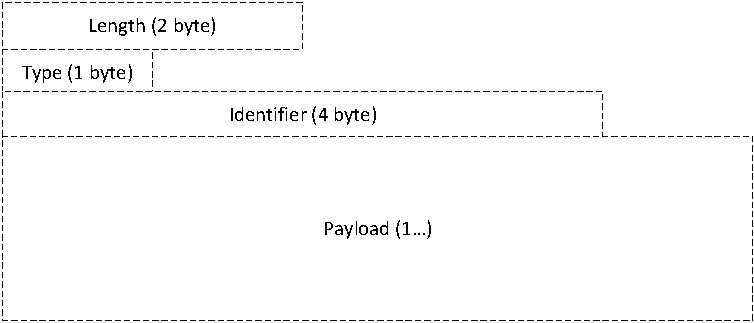
\includegraphics[width=\textwidth]{frames/framing.pdf}
\caption{Framing}
\label{framing}
\end{figure}

\section{Frames}

\subsection{Download Request}

A client sends this frame to the server to initiate a new download
or continue a paused download. In case of a new download the SHA1
hash must be set to all zeros. For paused downloads the SHA1 hash
must be set to the hash of the whole file, as opposed to the
hash of the already downloaded data. The filename is a sequence
of US ASCII characters, where the last character must be followed
by a zero. The identifier on this frame must always be set to zero. 

\begin{figure}[H]
\centering
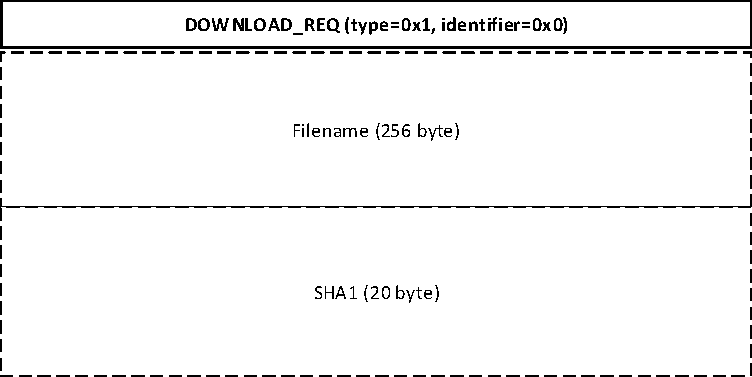
\includegraphics[width=\textwidth]{frames/download-req.pdf}
\caption{Download Request}
\label{DOWNLOAD-REQ}
\end{figure}

\subsection{Download Response}

A server responds with this frame to a download request from the
client. The frame has a random four byte identifier set, that
uniquely identifies this download. If the status is non-zero, 
then the download cannot be
started. The detailed semantics of each status code are outlined
in the status code section. The port specifies on which port to
send any subsequent frames with this identifier.

\begin{figure}[H]
\centering
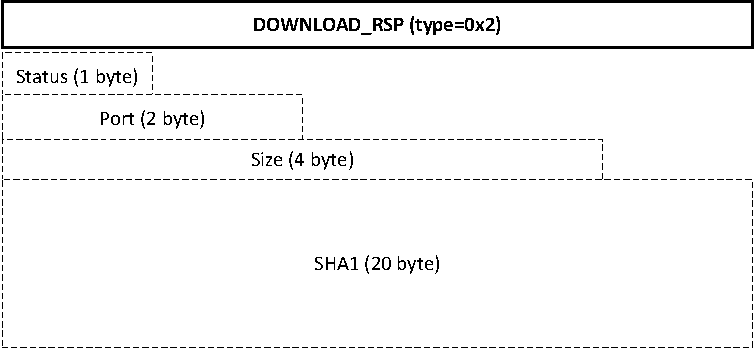
\includegraphics[width=\textwidth]{frames/download-rsp.pdf}
\caption{Download Response}
\label{DOWNLOAD-RSP}
\end{figure}

\subsection{Upload Request}

\begin{figure}[H]
\centering
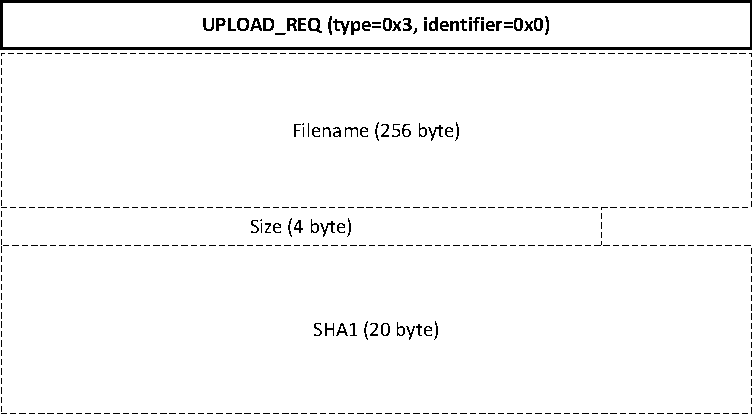
\includegraphics[width=\textwidth]{frames/upload-req.pdf}
\caption{Upload Request}
\label{UPLOAD-REQ}
\end{figure}

\subsection{Upload Response}

\begin{figure}[H]
\centering
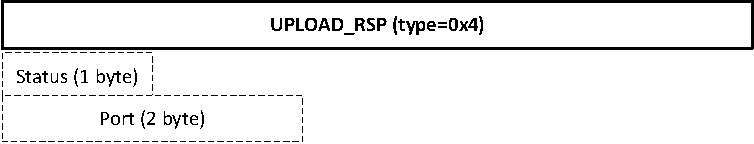
\includegraphics[width=\textwidth]{frames/upload-rsp.pdf}
\caption{Upload Response}
\label{UPLOAD-RSP}
\end{figure}

\subsection{Data Request}

In case of a download the client sends this frame to the
server, and in case of an upload the server sends this
frame to the client. This frame allows an endpoint to 
request a sequence of bytes of a given length at a specific
byte offset in a file. This frame also acts as an inbound
flow control mechanism for the receiving side. A data 
request may be answered by one or multiple data response
frames.

\begin{figure}[H]
\centering
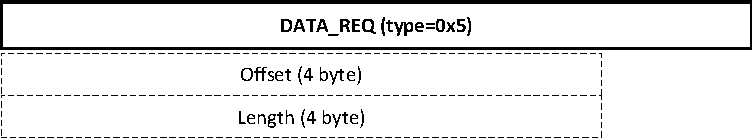
\includegraphics[width=\textwidth]{frames/data-req.pdf}
\caption{Data Request}
\label{DATA-REQ}
\end{figure}

\subsection{Data Response}

A data response frame may only be sent in response to a data
request frame.  

\begin{figure}[H]
\centering
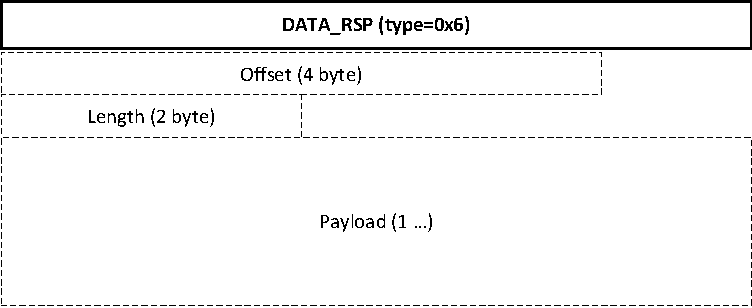
\includegraphics[width=\textwidth]{frames/data-rsp.pdf}
\caption{Data Response}
\label{DATA-RSP}
\end{figure}

\subsection{Checksum Request}

\begin{figure}[H]
\centering
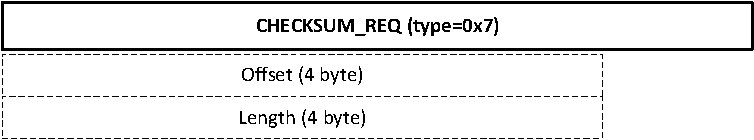
\includegraphics[width=\textwidth]{frames/checksum-req.pdf}
\caption{Checksum Request}
\label{CHECKSUM-REQ}
\end{figure}

\subsection{Checksum Response}

\begin{figure}[H]
\centering
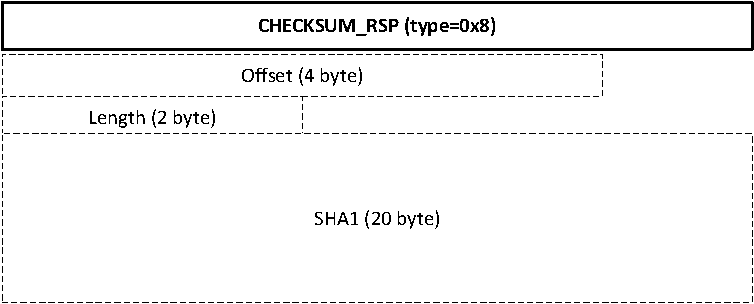
\includegraphics[width=\textwidth]{frames/checksum-rsp.pdf}
\caption{Checksum Response}
\label{CHECKSUM-RSP}
\end{figure}

\subsection{Termination Request}

This frame can be send bei either side of an upload and
download and at any point in time. After receiving
a termination request frame an endpoint needs to make a best
effort to stop any communication for the given identifier.
Any frames received after a termination request may be dropped.

\begin{figure}[H]
\centering
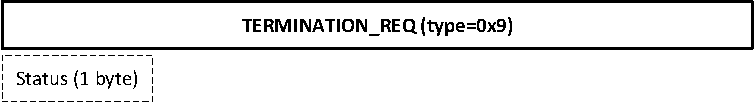
\includegraphics[width=\textwidth]{frames/shutdown-req.pdf}
\caption{Termination Request}
\label{TERMINATION-REQ}
\end{figure}

\section{Example Download}


\begin{figure}[H]
\centering
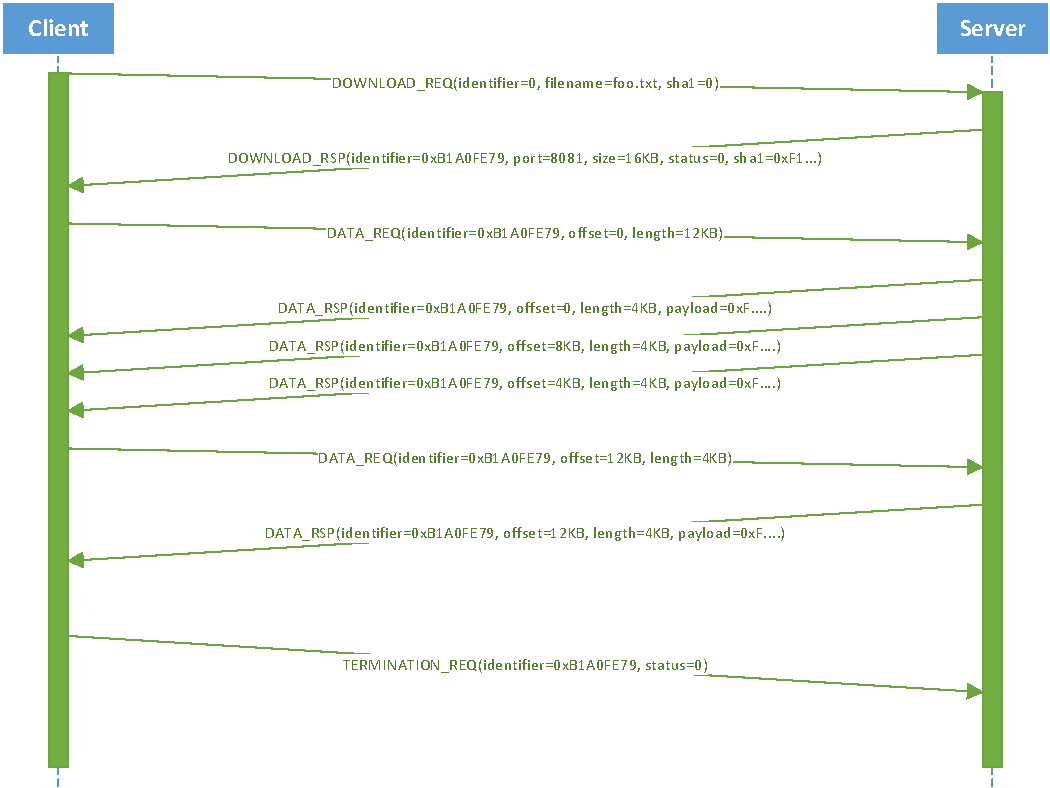
\includegraphics[width=\textwidth]{frames/download-interaction.pdf}
\caption{Example Download}
\label{EXAMPLE-DOWNLOAD}
\end{figure}


\end{document}
